
%% bare_conf.tex
%% V1.3
%% 2007/01/11
%% by Michael Shell
%% See:
%% http://www.michaelshell.org/
%% for current contact information.
%%
%% This is a skeleton file demonstrating the use of IEEEtran.cls
%% (requires IEEEtran.cls version 1.7 or later) with an IEEE conference paper.
%%
%% Support sites:
%% http://www.michaelshell.org/tex/ieeetran/
%% http://www.ctan.org/tex-archive/macros/latex/contrib/IEEEtran/
%% and
%% http://www.ieee.org/

%%*************************************************************************
%% Legal Notice:
%% This code is offered as-is without any warranty either expressed or
%% implied; without even the implied warranty of MERCHANTABILITY or
%% FITNESS FOR A PARTICULAR PURPOSE!
%% User assumes all risk.
%% In no event shall IEEE or any contributor to this code be liable for
%% any damages or losses, including, but not limited to, incidental,
%% consequential, or any other damages, resulting from the use or misuse
%% of any information contained here.
%%
%% All comments are the opinions of their respective authors and are not
%% necessarily endorsed by the IEEE.
%%
%% This work is distributed under the LaTeX Project Public License (LPPL)
%% ( http://www.latex-project.org/ ) version 1.3, and may be freely used,
%% distributed and modified. A copy of the LPPL, version 1.3, is included
%% in the base LaTeX documentation of all distributions of LaTeX released
%% 2003/12/01 or later.
%% Retain all contribution notices and credits.
%% ** Modified files should be clearly indicated as such, including  **
%% ** renaming them and changing author support contact information. **
%%
%% File list of work: IEEEtran.cls, IEEEtran_HOWTO.pdf, bare_adv.tex,
%%                    bare_conf.tex, bare_jrnl.tex, bare_jrnl_compsoc.tex
%%*************************************************************************

% *** Authors should verify (and, if needed, correct) their LaTeX system  ***
% *** with the testflow diagnostic prior to trusting their LaTeX platform ***
% *** with production work. IEEE's font choices can trigger bugs that do  ***
% *** not appear when using other class files.                            ***
% The testflow support page is at:
% http://www.michaelshell.org/tex/testflow/



% Note that the a4paper option is mainly intended so that authors in
% countries using A4 can easily print to A4 and see how their papers will
% look in print - the typesetting of the document will not typically be
% affected with changes in paper size (but the bottom and side margins will).
% Use the testflow package mentioned above to verify correct handling of
% both paper sizes by the user's LaTeX system.
%
% Also note that the "draftcls" or "draftclsnofoot", not "draft", option
% should be used if it is desired that the figures are to be displayed in
% draft mode.
%
\documentclass[10pt, conference, compsocconf]{IEEEtran}
% Add the compsocconf option for Computer Society conferences.
%
% If IEEEtran.cls has not been installed into the LaTeX system files,
% manually specify the path to it like:
% \documentclass[conference]{../sty/IEEEtran}





% Some very useful LaTeX packages include:
% (uncomment the ones you want to load)
\usepackage{color}
\usepackage{colortbl}

\definecolor{lightgray}{gray}{.95}
\definecolor{darkgray}{gray}{.80}

\usepackage{epsfig}
\usepackage{listings}

\lstset{ %
lineskip=0.5pt,
basicstyle=\scriptsize,       % the size of the fonts that are used for the code
%numbers=left,                   % where to put the line-numbers
numberstyle=\scriptsize,      % the size of the fonts that are used for the line-numbers
stepnumber=1,                   % the step between two line-numbers. If it is 1 each line will be numbered
numbersep=3pt,                  % how far the line-numbers are from the code
backgroundcolor=\color{lightgray},  % choose the background color. You must add \usepackage{color}
showspaces=false,               % show spaces adding particular underscores
showstringspaces=false,         % underline spaces within strings
showtabs=false,                 % show tabs within strings adding particular underscores
frame=none,                   % adds a frame around the code
tabsize=2,              % sets default tabsize to 2 spaces
captionpos=b,                   % sets the caption-position to bottom
breaklines=true,        % sets automatic line breaking
breakatwhitespace=false,    % sets if automatic breaks should only happen at whitespace
escapeinside={\%}{)}          % if you want to add a comment within your code
}


% *** MISC UTILITY PACKAGES ***
%
%\usepackage{ifpdf}
% Heiko Oberdiek's ifpdf.sty is very useful if you need conditional
% compilation based on whether the output is pdf or dvi.
% usage:
% \ifpdf
%   % pdf code
% \else
%   % dvi code
% \fi
% The latest version of ifpdf.sty can be obtained from:
% http://www.ctan.org/tex-archive/macros/latex/contrib/oberdiek/
% Also, note that IEEEtran.cls V1.7 and later provides a builtin
% \ifCLASSINFOpdf conditional that works the same way.
% When switching from latex to pdflatex and vice-versa, the compiler may
% have to be run twice to clear warning/error messages.






% *** CITATION PACKAGES ***
%
\usepackage{cite}
% cite.sty was written by Donald Arseneau
% V1.6 and later of IEEEtran pre-defines the format of the cite.sty package
% \cite{} output to follow that of IEEE. Loading the cite package will
% result in citation numbers being automatically sorted and properly
% "compressed/ranged". e.g., [1], [9], [2], [7], [5], [6] without using
% cite.sty will become [1], [2], [5]--[7], [9] using cite.sty. cite.sty's
% \cite will automatically add leading space, if needed. Use cite.sty's
% noadjust option (cite.sty V3.8 and later) if you want to turn this off.
% cite.sty is already installed on most LaTeX systems. Be sure and use
% version 4.0 (2003-05-27) and later if using hyperref.sty. cite.sty does
% not currently provide for hyperlinked citations.
% The latest version can be obtained at:
% http://www.ctan.org/tex-archive/macros/latex/contrib/cite/
% The documentation is contained in the cite.sty file itself.






% *** GRAPHICS RELATED PACKAGES ***
%
\ifCLASSINFOpdf
  % \usepackage[pdftex]{graphicx}
  % declare the path(s) where your graphic files are
  % \graphicspath{{../pdf/}{../jpeg/}}
  % and their extensions so you won't have to specify these with
  % every instance of \includegraphics
  % \DeclareGraphicsExtensions{.pdf,.jpeg,.png}
\else
  % or other class option (dvipsone, dvipdf, if not using dvips). graphicx
  % will default to the driver specified in the system graphics.cfg if no
  % driver is specified.
  % \usepackage[dvips]{graphicx}
  % declare the path(s) where your graphic files are
  % \graphicspath{{../eps/}}
  % and their extensions so you won't have to specify these with
  % every instance of \includegraphics
  % \DeclareGraphicsExtensions{.eps}
\fi
% graphicx was written by David Carlisle and Sebastian Rahtz. It is
% required if you want graphics, photos, etc. graphicx.sty is already
% installed on most LaTeX systems. The latest version and documentation can
% be obtained at:
% http://www.ctan.org/tex-archive/macros/latex/required/graphics/
% Another good source of documentation is "Using Imported Graphics in
% LaTeX2e" by Keith Reckdahl which can be found as epslatex.ps or
% epslatex.pdf at: http://www.ctan.org/tex-archive/info/
%
% latex, and pdflatex in dvi mode, support graphics in encapsulated
% postscript (.eps) format. pdflatex in pdf mode supports graphics
% in .pdf, .jpeg, .png and .mps (metapost) formats. Users should ensure
% that all non-photo figures use a vector format (.eps, .pdf, .mps) and
% not a bitmapped formats (.jpeg, .png). IEEE frowns on bitmapped formats
% which can result in "jaggedy"/blurry rendering of lines and letters as
% well as large increases in file sizes.
%
% You can find documentation about the pdfTeX application at:
% http://www.tug.org/applications/pdftex





% *** MATH PACKAGES ***
%
%\usepackage[cmex10]{amsmath}
% A popular package from the American Mathematical Society that provides
% many useful and powerful commands for dealing with mathematics. If using
% it, be sure to load this package with the cmex10 option to ensure that
% only type 1 fonts will utilized at all point sizes. Without this option,
% it is possible that some math symbols, particularly those within
% footnotes, will be rendered in bitmap form which will result in a
% document that can not be IEEE Xplore compliant!
%
% Also, note that the amsmath package sets \interdisplaylinepenalty to 10000
% thus preventing page breaks from occurring within multiline equations. Use:
%\interdisplaylinepenalty=2500
% after loading amsmath to restore such page breaks as IEEEtran.cls normally
% does. amsmath.sty is already installed on most LaTeX systems. The latest
% version and documentation can be obtained at:
% http://www.ctan.org/tex-archive/macros/latex/required/amslatex/math/





% *** SPECIALIZED LIST PACKAGES ***
%
%\usepackage{algorithmic}
% algorithmic.sty was written by Peter Williams and Rogerio Brito.
% This package provides an algorithmic environment fo describing algorithms.
% You can use the algorithmic environment in-text or within a figure
% environment to provide for a floating algorithm. Do NOT use the algorithm
% floating environment provided by algorithm.sty (by the same authors) or
% algorithm2e.sty (by Christophe Fiorio) as IEEE does not use dedicated
% algorithm float types and packages that provide these will not provide
% correct IEEE style captions. The latest version and documentation of
% algorithmic.sty can be obtained at:
% http://www.ctan.org/tex-archive/macros/latex/contrib/algorithms/
% There is also a support site at:
% http://algorithms.berlios.de/index.html
% Also of interest may be the (relatively newer and more customizable)
% algorithmicx.sty package by Szasz Janos:
% http://www.ctan.org/tex-archive/macros/latex/contrib/algorithmicx/




% *** ALIGNMENT PACKAGES ***
%
%\usepackage{array}
% Frank Mittelbach's and David Carlisle's array.sty patches and improves
% the standard LaTeX2e array and tabular environments to provide better
% appearance and additional user controls. As the default LaTeX2e table
% generation code is lacking to the point of almost being broken with
% respect to the quality of the end results, all users are strongly
% advised to use an enhanced (at the very least that provided by array.sty)
% set of table tools. array.sty is already installed on most systems. The
% latest version and documentation can be obtained at:
% http://www.ctan.org/tex-archive/macros/latex/required/tools/


%\usepackage{mdwmath}
%\usepackage{mdwtab}
% Also highly recommended is Mark Wooding's extremely powerful MDW tools,
% especially mdwmath.sty and mdwtab.sty which are used to format equations
% and tables, respectively. The MDWtools set is already installed on most
% LaTeX systems. The lastest version and documentation is available at:
% http://www.ctan.org/tex-archive/macros/latex/contrib/mdwtools/


% IEEEtran contains the IEEEeqnarray family of commands that can be used to
% generate multiline equations as well as matrices, tables, etc., of high
% quality.


%\usepackage{eqparbox}
% Also of notable interest is Scott Pakin's eqparbox package for creating
% (automatically sized) equal width boxes - aka "natural width parboxes".
% Available at:
% http://www.ctan.org/tex-archive/macros/latex/contrib/eqparbox/





% *** SUBFIGURE PACKAGES ***
%\usepackage[tight,footnotesize]{subfigure}
% subfigure.sty was written by Steven Douglas Cochran. This package makes it
% easy to put subfigures in your figures. e.g., "Figure 1a and 1b". For IEEE
% work, it is a good idea to load it with the tight package option to reduce
% the amount of white space around the subfigures. subfigure.sty is already
% installed on most LaTeX systems. The latest version and documentation can
% be obtained at:
% http://www.ctan.org/tex-archive/obsolete/macros/latex/contrib/subfigure/
% subfigure.sty has been superceeded by subfig.sty.



%\usepackage[caption=false]{caption}
%\usepackage[font=footnotesize]{subfig}
% subfig.sty, also written by Steven Douglas Cochran, is the modern
% replacement for subfigure.sty. However, subfig.sty requires and
% automatically loads Axel Sommerfeldt's caption.sty which will override
% IEEEtran.cls handling of captions and this will result in nonIEEE style
% figure/table captions. To prevent this problem, be sure and preload
% caption.sty with its "caption=false" package option. This is will preserve
% IEEEtran.cls handing of captions. Version 1.3 (2005/06/28) and later
% (recommended due to many improvements over 1.2) of subfig.sty supports
% the caption=false option directly:
%\usepackage[caption=false,font=footnotesize]{subfig}
%
% The latest version and documentation can be obtained at:
% http://www.ctan.org/tex-archive/macros/latex/contrib/subfig/
% The latest version and documentation of caption.sty can be obtained at:
% http://www.ctan.org/tex-archive/macros/latex/contrib/caption/




% *** FLOAT PACKAGES ***
%
%\usepackage{fixltx2e}
% fixltx2e, the successor to the earlier fix2col.sty, was written by
% Frank Mittelbach and David Carlisle. This package corrects a few problems
% in the LaTeX2e kernel, the most notable of which is that in current
% LaTeX2e releases, the ordering of single and double column floats is not
% guaranteed to be preserved. Thus, an unpatched LaTeX2e can allow a
% single column figure to be placed prior to an earlier double column
% figure. The latest version and documentation can be found at:
% http://www.ctan.org/tex-archive/macros/latex/base/



%\usepackage{stfloats}
% stfloats.sty was written by Sigitas Tolusis. This package gives LaTeX2e
% the ability to do double column floats at the bottom of the page as well
% as the top. (e.g., "\begin{figure*}[!b]" is not normally possible in
% LaTeX2e). It also provides a command:
%\fnbelowfloat
% to enable the placement of footnotes below bottom floats (the standard
% LaTeX2e kernel puts them above bottom floats). This is an invasive package
% which rewrites many portions of the LaTeX2e float routines. It may not work
% with other packages that modify the LaTeX2e float routines. The latest
% version and documentation can be obtained at:
% http://www.ctan.org/tex-archive/macros/latex/contrib/sttools/
% Documentation is contained in the stfloats.sty comments as well as in the
% presfull.pdf file. Do not use the stfloats baselinefloat ability as IEEE
% does not allow \baselineskip to stretch. Authors submitting work to the
% IEEE should note that IEEE rarely uses double column equations and
% that authors should try to avoid such use. Do not be tempted to use the
% cuted.sty or midfloat.sty packages (also by Sigitas Tolusis) as IEEE does
% not format its papers in such ways.



\usepackage{boxedminipage}
\usepackage{graphicx}

\newcommand{\notesbox}[1]{
%     \ \\
      \noindent\begin{center}\begin{boxedminipage}[h]{0.4\textwidth}{#1}\end{boxedminipage}\end{center}
}

% *** PDF, URL AND HYPERLINK PACKAGES ***
%
%\usepackage{url}
% url.sty was written by Donald Arseneau. It provides better support for
% handling and breaking URLs. url.sty is already installed on most LaTeX
% systems. The latest version can be obtained at:
% http://www.ctan.org/tex-archive/macros/latex/contrib/misc/
% Read the url.sty source comments for usage information. Basically,
% \url{my_url_here}.





% *** Do not adjust lengths that control margins, column widths, etc. ***
% *** Do not use packages that alter fonts (such as pslatex).         ***
% There should be no need to do such things with IEEEtran.cls V1.6 and later.
% (Unless specifically asked to do so by the journal or conference you plan
% to submit to, of course. )


% correct bad hyphenation here
\hyphenation{op-tical net-works semi-conduc-tor}


\begin{document}
%
% paper title
% can use linebreaks \\ within to get better formatting as desired
\title{Automatic Repair of Concurrency Bugs}


% author names and affiliations
% use a multiple column layout for up to two different
% affiliations

\author{\IEEEauthorblockN{Jeremy S. Bradbury, Kevin Jalbert}
\IEEEauthorblockA{Software Quality Research Group\\
Faculty of Science (Computer Science)\\
University of Ontario Institute of Technology\\
Oshawa, Ontario, Canada\\
\{jeremy.bradbury, kevin.jalbert\}@uoit.ca}
}

% conference papers do not typically use \thanks and this command
% is locked out in conference mode. If really needed, such as for
% the acknowledgment of grants, issue a \IEEEoverridecommandlockouts
% after \documentclass

% for over three affiliations, or if they all won't fit within the width
% of the page, use this alternative format:
%
%\author{\IEEEauthorblockN{Michael Shell\IEEEauthorrefmark{1},
%Homer Simpson\IEEEauthorrefmark{2},
%James Kirk\IEEEauthorrefmark{3},
%Montgomery Scott\IEEEauthorrefmark{3} and
%Eldon Tyrell\IEEEauthorrefmark{4}}
%\IEEEauthorblockA{\IEEEauthorrefmark{1}School of Electrical and Computer Engineering\\
%Georgia Institute of Technology,
%Atlanta, Georgia 30332--0250\\ Email: see http://www.michaelshell.org/contact.html}
%\IEEEauthorblockA{\IEEEauthorrefmark{2}Twentieth Century Fox, Springfield, USA\\
%Email: homer@thesimpsons.com}
%\IEEEauthorblockA{\IEEEauthorrefmark{3}Starfleet Academy, San Francisco, California 96678-2391\\
%Telephone: (800) 555--1212, Fax: (888) 555--1212}
%\IEEEauthorblockA{\IEEEauthorrefmark{4}Tyrell Inc., 123 Replicant Street, Los Angeles, California 90210--4321}}




% use for special paper notices
%\IEEEspecialpapernotice{(Invited Paper)}




% make the title area
\maketitle


\begin{abstract}
Bugs in concurrent software are difficult to identify and fix since they may only exhibit abnormal behaviour on certain thread interleavings. We propose the use of genetic programming to incrementally create a solution that fixes a concurrency bug automatically. Bugs in a concurrent program are fixed by iteratively mutating the program and evaluating each mutation using a fitness function that compares the mutated program with the previous version. We propose three mutation operators that can fix concurrency bugs: synchronize an unprotected shared resource, expand synchronization regions to include unprotected source code, and interchange nested lock objects.
%Bugs in concurrent software are difficult to identify and fix since they may only exhibit abnormal behaviour on certain thread interleavings. Genetic algorithms are extremely useful at solving optimization and search-based problems. By using genetic algorithms we implement an approach to incrementally create a solution that fixes a bug automatically. A bug fix is formed by iteratively mutating the program and evaluating the mutation using a fitness function that test for the bug's existence. We have identified three types of mutation operations that can fix concurrency bugs: synchronize an unprotected shared resource, expand synchronization regions to include unprotected source code, and interchanging nested lock objects. We believe our algorithm can at least partially fix the bug and guide the developer in the correct direction.

\end{abstract}

\begin{IEEEkeywords}
concurrency; genetic programming; mutation.

\end{IEEEkeywords}


% For peer review papers, you can put extra information on the cover
% page as needed:
% \ifCLASSOPTIONpeerreview
% \begin{center} \bfseries EDICS Category: 3-BBND \end{center}
% \fi
%
% For peerreview papers, this IEEEtran command inserts a page break and
% creates the second title. It will be ignored for other modes.
\IEEEpeerreviewmaketitle



\section{Introduction}
\label{sec:introduction}

Concurrency bugs are difficult and expensive to fix since there are often many interleavings for a concurrent program. We propose using a search-based technique, specifically genetic programming, to apply and assess possible fixes for common concurrency bugs. In particular we are interested in fixing deadlocks and data races. A deadlock occurs in  \emph{``...a situation where two or more processes are unable to proceed because each is waiting for one of the others to do something...''}~\cite{LSW05}. A data race occurs when \emph{``...two or more concurrent threads access a shared variable and when at least one access is a write, and the threads use no explicit mechanism to prevent the access from being simultaneous''}~\cite{LSW05}.

There has been a great deal of research in the area of search-based software engineering~\cite{Har+10}. Furthermore, the use of genetic programming to aid in identifying a solution that fixes a bug is not a novel idea~\cite{FNWG09, AY08, Arc08, WT10, WNLF09, WFGN10}. Our proposed approach adapts the original idea of automatically fixing sequential software using genetic programming to specifically target concurrent software. Bugs in a concurrent program are fixed by iteratively mutating the program and evaluating each mutation using a fitness function that compares the mutated program with the previous version. We have focused on deadlock and data race bugs and have identified three mutation operators that can insert potential fixes into a concurrent program. We believe that this approach can be very successful with respect to concurrency bugs since the possible set of fixes is relatively small and the possible fixes are limited to source code locations associated with access to shared data and the protection of shared data. In the previous research using genetic programming to fix bugs in sequential programs, the general approach has proved successful with a larger set of possible actions and thus suggests that the correction of concurrent software is also feasible.

To the best of our knowledge there has been no previous work using genetic programming to patch bugs in concurrent software, However, there has also been work that involves the correction of concurrency bugs using self-healing~\cite{LVK08}. The self-healing approach is applied dynamically and is focused on coping with a concurrency bug, while our approach evolves the source code in order to correct the bug.

%In the next section we will explain our approach and outline our mutation operators and the fitness function used in our genetic programming approach. In the final section we will present our initial conclusions and discuss several possible avenues of future work.

\section{Our Automatic Repair Process}
\label{sec:genetic_algorithm}

%Genetic algorithms are well defined and requires the following concepts: input data, mutation operators, fitness function, and terminating conditions. Each of these concepts must be tailored specifically to automatically repair concurrency bugs. Our approach is described in the following sections.

\begin{figure}[!t]
\centering
%\hrule
%\vspace{2mm}
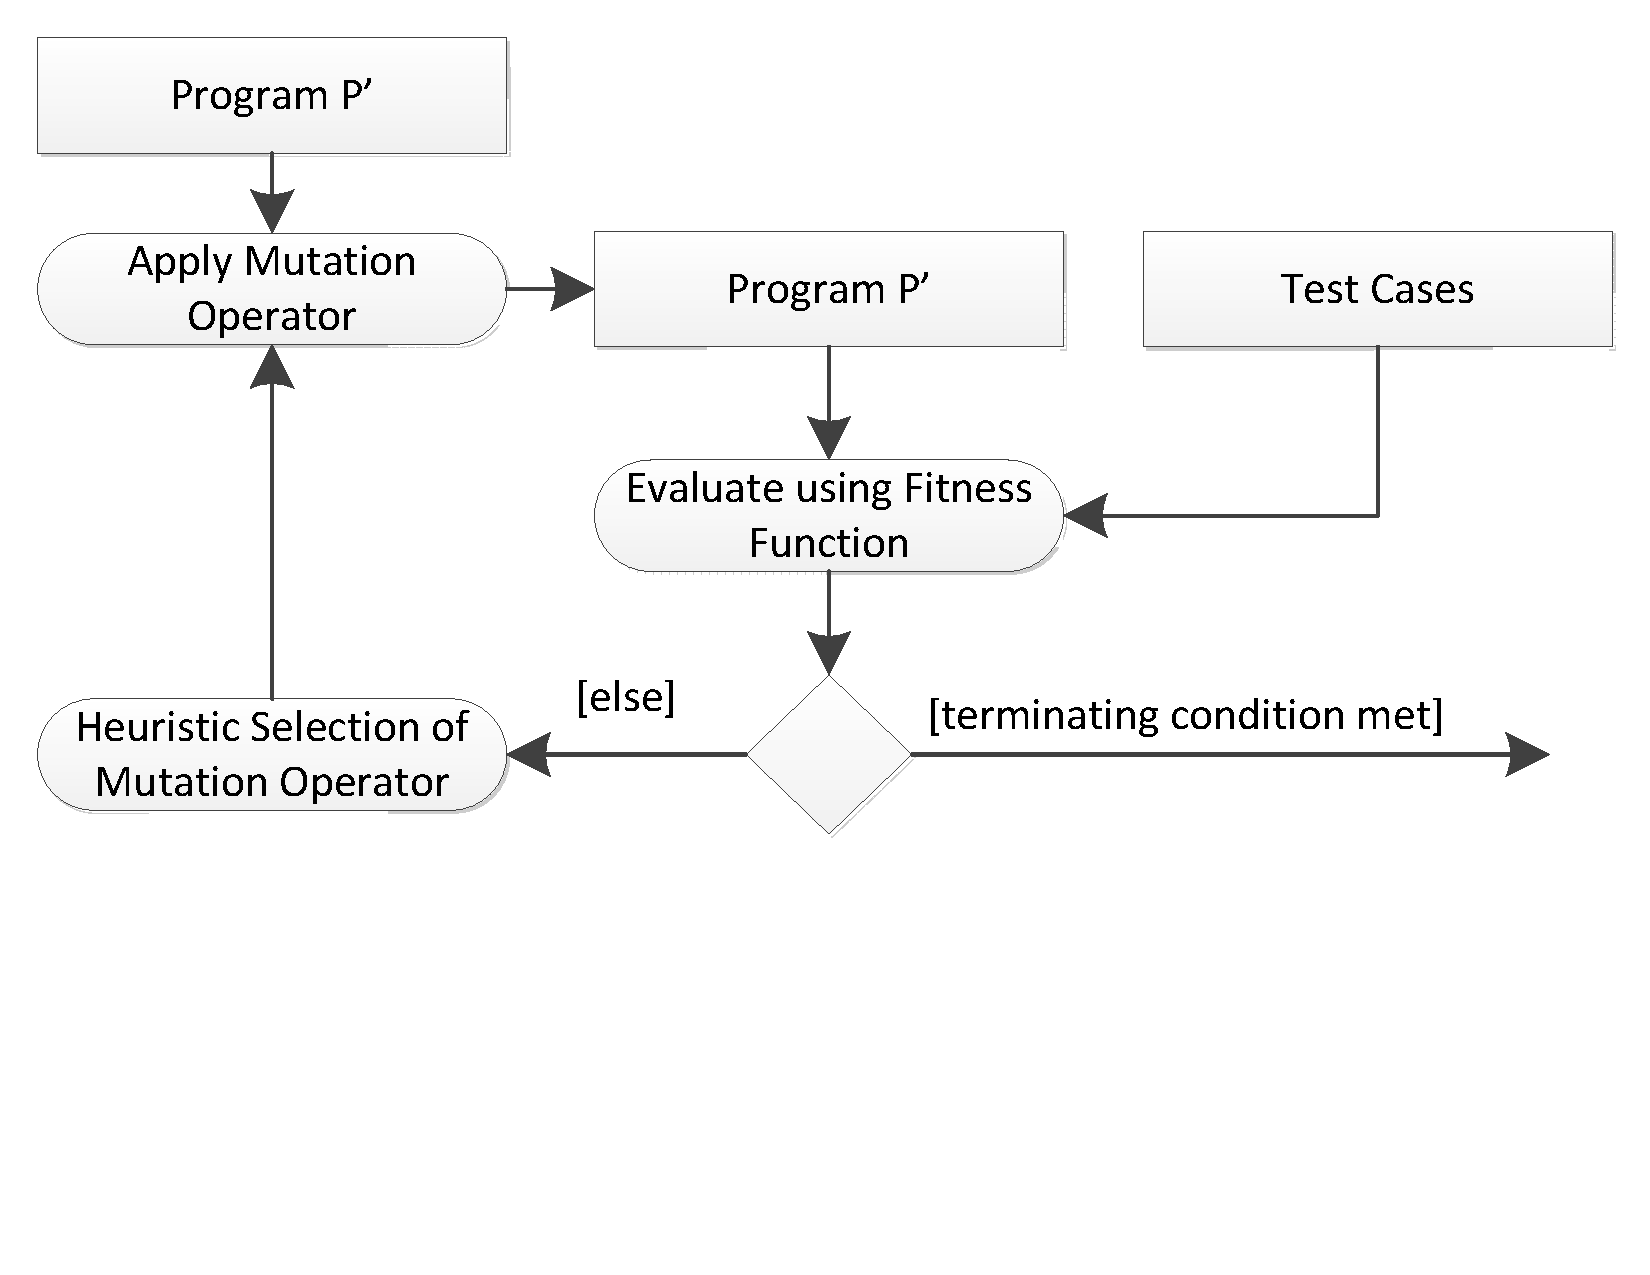
\includegraphics[width=6.7cm]{figures/process.pdf}
\caption{Automatic Repair Process}
\label{fig:process}
%\vspace{1mm}
%\footnotesize{\emph{Legend: Rounded grey rectangles represent process phase. White rectangles with a folded corner represent data input. Diamond represents a decision.}}
%\vspace{2mm}
%\hrule
\end{figure}

Our process expects a concurrent program $P$ as input (see Figure~\ref{fig:process}). A mutation operator is applied to $P$, which results in a mutated program, $P'$. We have identified three mutation operators that can correct data race and deadlock bugs. We have previously explored variations of these operators in previous work on mutation testing of concurrent software~\cite{BCD06b}. %The operators are applied to the source tree of the program due to the nature of how concurrency is written (by encapsulating regions of source code in synchronizations).
The first two operators specifically target data race bugs while the third operator targets deadlock bugs:%\footnote{It must be noted that by applying these mutations it might be possible to induce new deadlock bugs.}:

\begin{enumerate}
	\item \textit{Synchronize an unprotected shared resource.} One cause of a data race is that a shared resource is unprotected. By synchronizing around a shared resource data races can be fixed.

\vspace{2mm}
	\begin{minipage}{3.70cm}
	\footnotesize{\textbf{ Program $P$:}}
\begin{lstlisting}[language=Java]
...
obj.write( var1 );
...

\end{lstlisting}
\end{minipage}\hfill
\begin{minipage}{3.70cm}
\footnotesize{\textbf{ Program $P'$:}}
\begin{lstlisting}[language=Java]
synchronized ( lock ){
	obj.write( var1 );
}
\end{lstlisting}
\end{minipage}


	\item \textit{Expand synchronization regions to include unprotected source code.} Data races can sometimes be caused if the synchronization region does not fully encapsulate access to the shared resources. Expanding the synchronization region can also fix the data race.

\vspace{2mm}
	\begin{minipage}{3.70cm}
\footnotesize{\textbf{ Program $P$:}}
\begin{lstlisting}[language=Java]
synchronized ( lock ){
	obj.write( var1 );
}
obj.write( var2 );
\end{lstlisting}
\end{minipage}\hfill
\begin{minipage}{3.70cm}
\footnotesize{\textbf{ Program $P'$:}}
\begin{lstlisting}[language=Java]
synchronized ( lock ){
	obj.write( var1 );
	obj.write( var2 );
}
\end{lstlisting}
\end{minipage}


	\item \textit{Interchange nested lock objects.} Common deadlocks occur due to the ordering of lock acquisition. By interchanging nested lock objects common deadlocks can be fixed.

\vspace{2mm}
	\begin{minipage}{3.70cm}
\footnotesize{\textbf{ Program $P$:}}
\begin{lstlisting}[language=Java]
synchronized ( lock1 ){
	synchronized ( lock2 ){
		obj.write( var1 );
	}
}
\end{lstlisting}
\end{minipage}\hfill
\begin{minipage}{3.70cm}
\footnotesize{\textbf{ Program $P'$:}}
\begin{lstlisting}[language=Java]
synchronized ( lock2 ){
	synchronized ( lock1 ){
		obj.write( var1 );
	}
}
\end{lstlisting}
\end{minipage}

\end{enumerate}

After the application of a mutation operator, the new program, $P'$, is then evaluated using our fitness function:

%\notesbox{
\begin{footnotesize}
\begin{center}
$fitness(P) = \displaystyle\sum\limits_{i=0}^n\frac{interleavings\ without\ a\ bug}{total\ \#\ of\ interleavings\ tested}$
\end{center}
\end{footnotesize}
\begin{tiny}
\begin{center}
$n = \#\ of\ Test\ Cases$
\end{center}
\end{tiny}
%}

Our fitness function differs from the function used by Weimer et al. in which the fitness is the weighted value of the number of tests that pass in addition to a weighted sum of the number of tests that fail. Since we are focused on concurrent programs we have to provide coverage of the interleaving space and need to run each test many times in order to provide confidence that the test will not fail for some interleaving. Therefore, we have chosen to calculate the percent of interleavings that pass for each test case and use the sum of these values as our measure of fitness. We evaluate our fitness function by running all tests with $P'$ a number of times using a concurrency testing tool (e.g., IBM's ConTest~\cite{EFN+02}) to aid in exploring different thread interleavings.  If the $fitness(P') > fitness(P)$ then a given mutation is kept, otherwise it is discarded.%The scoring of the new programs will be the summation of the percentages of interleavings that causes a bug for each test case.


We next check if the process can terminate or if more mutations (i.e., bug fixes) are required. The terminating conditions are: (1) a program $P'$ has reached a user-defined threshold of success meaning that enough tests succeed with enough interleavings to provide confidence in the program correctness, (2) the process has progressed a predefined number of iterations without significant progress.

If no terminating condition is met then we need to select a mutation operator for the next iteration of the algorithm. We do not select the mutation operators randomly. Instead, we select mutations based on the bugs present in the program. For example, if most of the test cases failed due to a deadlock then selecting the third mutation operator has the best chance of fixing the deadlock otherwise we select one of the other two operators.

For simplicity, our process was described with one mutation per iteration. Ideally, we can mutate the program to generate and evaluate multiple mutants per iteration in order to find a solution more quickly.

\section{Conclusion \& Future Work}
\label{sec:conclusion_future_work}

Genetic programming has been used to fix sequential programs~\cite{FNWG09, AY08, Arc08, WNLF09, WFGN10} and additional work has focused on refinement of this approach~\cite{WT10}. Our research is an adaptation of this previous work that targets concurrent programs with deadlock and data race bugs. Currently, we are in the process of implementing our work.  After the implementation is complete we plan to evaluate and refine many aspects of our approach including: the mutation operators, the fitness function, the termination threshold and the heuristic selection of mutation operators.

% use section* for acknowledgement
%\section*{Acknowledgment}
%The authors would like to thank the Natural Sciences and Engineering Research Council of Canada (NSERC) for funding this research.


% trigger a \newpage just before the given reference
% number - used to balance the columns on the last page
% adjust value as needed - may need to be readjusted if
% the document is modified later
%\IEEEtriggeratref{8}
% The "triggered" command can be changed if desired:
%\IEEEtriggercmd{\enlargethispage{-5in}}

% references section

% can use a bibliography generated by BibTeX as a .bbl file
% BibTeX documentation can be easily obtained at:
% http://www.ctan.org/tex-archive/biblio/bibtex/contrib/doc/
% The IEEEtran BibTeX style support page is at:
% http://www.michaelshell.org/tex/ieeetran/bibtex/
\bibliographystyle{IEEEtran}
% argument is your BibTeX string definitions and bibliography database(s)
\bibliography{SSBSE2010.bib}
%
% <OR> manually copy in the resultant .bbl file
% set second argument of \begin to the number of references
% (used to reserve space for the reference number labels box)




% that's all folks
\end{document}
